\chapter{Intro to Cyber Defense}
\newpage

\section*{Kickoff: RCE (Remote Code Execution)}
\subsection*{What is it?}
Remote Code Execution (RCE) refers to a security vulnerability that allows attackers to execute arbitrary code remotely on a target system. This can have very far-reaching consequences, as the attacker can perform almost any action on the compromised system.

\begin{itemize}
    \item Examples include Command Injection, File Upload (e.g., PHP file), SQL Injection, Buffer Overflow (custom code).
\end{itemize}

\subsection*{Requirements}
\begin{itemize}
    \item A vulnerable component (e.g., outdated library, unpatched software).
    \item Insufficient input validation, which allows malicious code to be injected (e.g., via insecure deserialization).
    \item Lack of security mechanisms (e.g., no WAF, no access restrictions).
\end{itemize}

\subsection*{Countermeasures}
\begin{itemize}
    \item Apply security updates and patches promptly.
    \item Use secure frameworks and implement thorough input validation.
    \item Secure systems using WAF (Web Application Firewall) and IDS/IPS.
    \item Apply the principle of least privilege: run services with only the minimum required permissions.
\end{itemize}

\begin{center}
    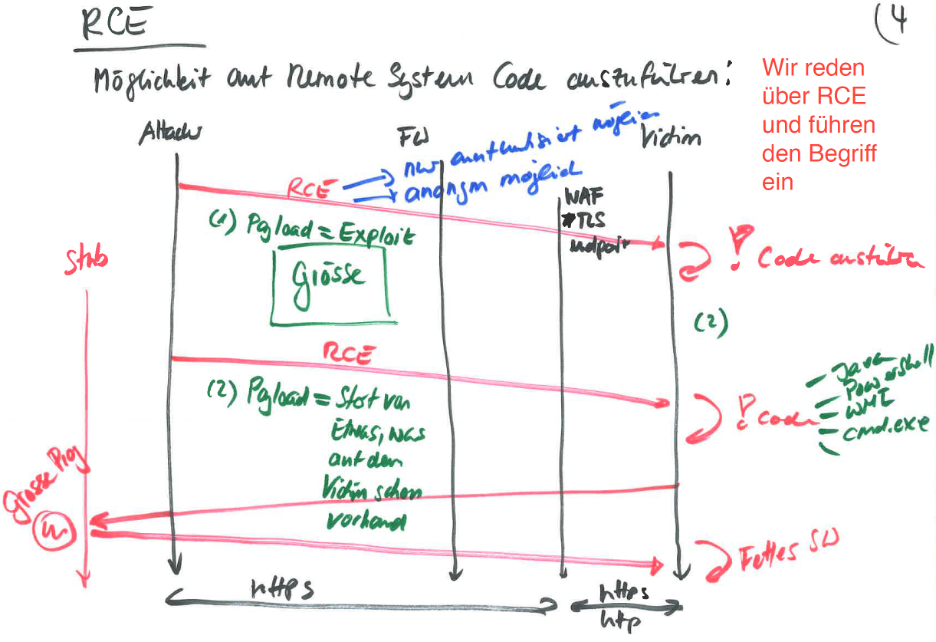
\includegraphics[scale=1]{resources/01_rce.png}
\end{center}

\section*{Log4J}
\subsection*{What is it?}
Log4J is a popular Java logging framework. The well-known vulnerability (“Log4Shell”) allowed attackers, under certain conditions, to execute remote code by processing manipulated inputs via JNDI (Java Naming and Directory Interface) calls.

\begin{center}
    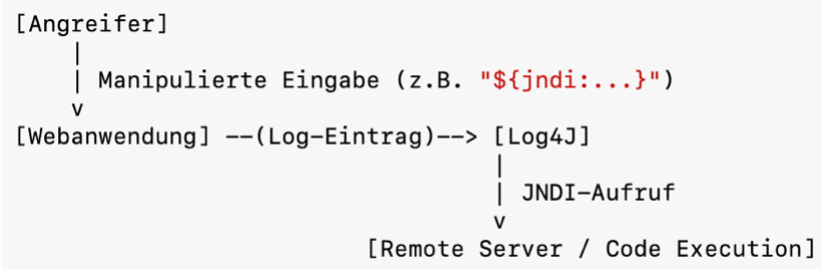
\includegraphics[scale=1]{resources/01_log4j.png}
\end{center}

\subsection*{Requirements}
\begin{itemize}
    \item Use of a vulnerable Log4J version (e.g., < 2.17 in many cases).
    \item Capability for the attacker to inject payloads processed by the Log4J logger.
    \item Enabled JNDI feature and missing security properties.
\end{itemize}

\subsection*{Countermeasures}
\begin{itemize}
    \item Update to a patched Log4J version (e.g., >= 2.17.1).
    \item Disable or secure JNDI lookups in Log4J configurations.
    \item Validate incoming data and filter potentially harmful strings.
\end{itemize}

\begin{center}
    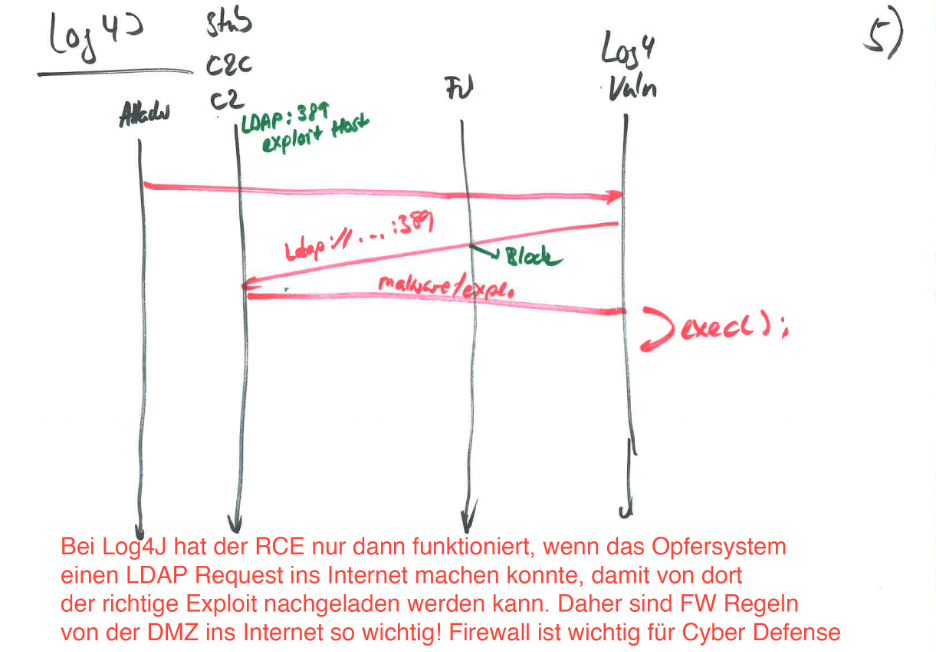
\includegraphics[scale=1]{resources/01_log4j_sequence.png}
\end{center}

\section*{CVE \& CWE}
\subsection*{What is it?}
\begin{itemize}
    \item \textbf{CVE} (Common Vulnerabilities and Exposures) is a standardized directory for known security vulnerabilities. Each vulnerability is assigned a unique CVE number (e.g., CVE-2021-XYZ).
    \item \textbf{CWE} (Common Weakness Enumeration) describes and classifies fundamental categories of software weaknesses (e.g., “CWE-79: Cross-Site Scripting”).
\end{itemize}

\begin{center}
    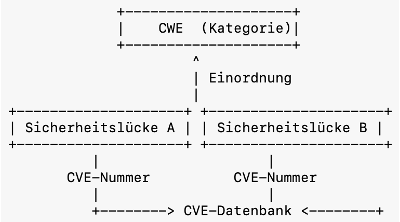
\includegraphics[scale=1]{resources/01_cve_cwe.png}
\end{center}

\subsection*{Requirements}
Requirements for CVE/CWE classification include the presence of an actual or potential vulnerability in a software/component.

\subsection*{Countermeasures}
\begin{itemize}
    \item Use CVE databases to quickly identify and patch known vulnerabilities.
    \item Use CWE classifications to detect and avoid vulnerabilities early in the development process.
    \item Continuously scan and test the software (SAST/DAST).
\end{itemize}

\section*{CORS (Cross-Origin Resource Sharing)}
\subsection*{What is it?}
CORS is a security mechanism in web browsers that regulates whether and how resources (e.g., APIs) from one domain can access another domain. Without CORS permissions, browsers block such requests by default for security reasons.

\begin{itemize}
    \item CORS does not prevent requests to the API from being made.
    \item CORS only prevents the response from being processed.
\end{itemize}

\subsection*{Requirements}
\begin{itemize}
    \item A web application that wants to load content or query data from other domains.
    \item A server that controls access permissions for foreign domains via CORS headers (e.g., \texttt{Access-Control-Allow-Origin}).
    \item A browser that enforces the CORS mechanism.
\end{itemize}

\subsection*{Countermeasures}
\begin{itemize}
    \item Carefully configure CORS headers (e.g., \texttt{Access-Control-Allow-Origin}, \texttt{Access-Control-Allow-Methods}, etc.).
    \item Use "allow lists" (white lists) for trusted domains.
    \item If needed, use token-based authentication to further secure access.
\end{itemize}

\subsection*{Where does permission come from?}
\begin{enumerate}
    \item \textbf{The server provides it:} The key factor is what the server sends back in its CORS headers.
    \item \textbf{The browser enforces it:} The browser performs the check. Even if the server sets incorrect headers, the browser blocks the request.
    \item \textbf{Configuration:} In most web servers or frameworks (e.g., Spring Boot, Express.js, NGINX), you can configure which domains, methods, and headers are allowed.
\end{enumerate}

\subsection*{Examples for \texttt{Access-Control-Allow-Origin}}
\begin{itemize}
    \item \texttt{Access-Control-Allow-Origin: https://my-site.com} $\rightarrow$ for a single site.
    \item \texttt{Access-Control-Allow-Origin: *} $\rightarrow$ for all.
\end{itemize}

\section{Exercise}

\section{CyberChef Overview}
CyberChef is a simple, intuitive web application for performing a variety of 'cyber' operations in a browser. These include:
\begin{itemize}
    \item Simple ciphers such as XOR and Base64.
    \item Complex ciphers such as AES, DES, and Blowfish.
    \item Creating binary and hex dumps.
    \item Compressing and decompressing data.
    \item Calculating hashes and checksums.
    \item Parsing IPv6 and X.509.
    \item Changing character encodings.
\end{itemize}

CyberChef was developed to allow both technical and non-technical analysts to manipulate data in complex ways without dealing with complex tools or algorithms. It has been incrementally improved by an analyst over several years.

\subsection{Key Features}
\begin{itemize}
    \item \textbf{Fork}: Splits the input data based on a specified delimiter and runs all subsequent operations on each branch separately.
    \item \textbf{Merge}: Consolidates all branches back into a single trunk. Unticking the \emph{Merge All} checkbox consolidates branches up to the nearest Fork/Subsection.
    \item \textbf{Register}: Extracts data from the input and stores it in registers, which can then be used as arguments in subsequent operations. Regular expression capture groups select the data to extract.
\end{itemize}

\subsection{Exercises and Solutions}

\subsubsection{Forking Example}
\textbf{Input:}
\begin{verbatim}
cas
cyber
security
\end{verbatim}

\textbf{Steps:}
\begin{enumerate}
    \item Used the \emph{Fork} tool with default parameters (split by newline character).
    \item Applied \emph{Generate All Hashes} operation on each branch.
\end{enumerate}

\textbf{Output:} Various hashes generated for each input. See Figure~\ref{fig:forking}.

\begin{figure}[h!]
    \centering
    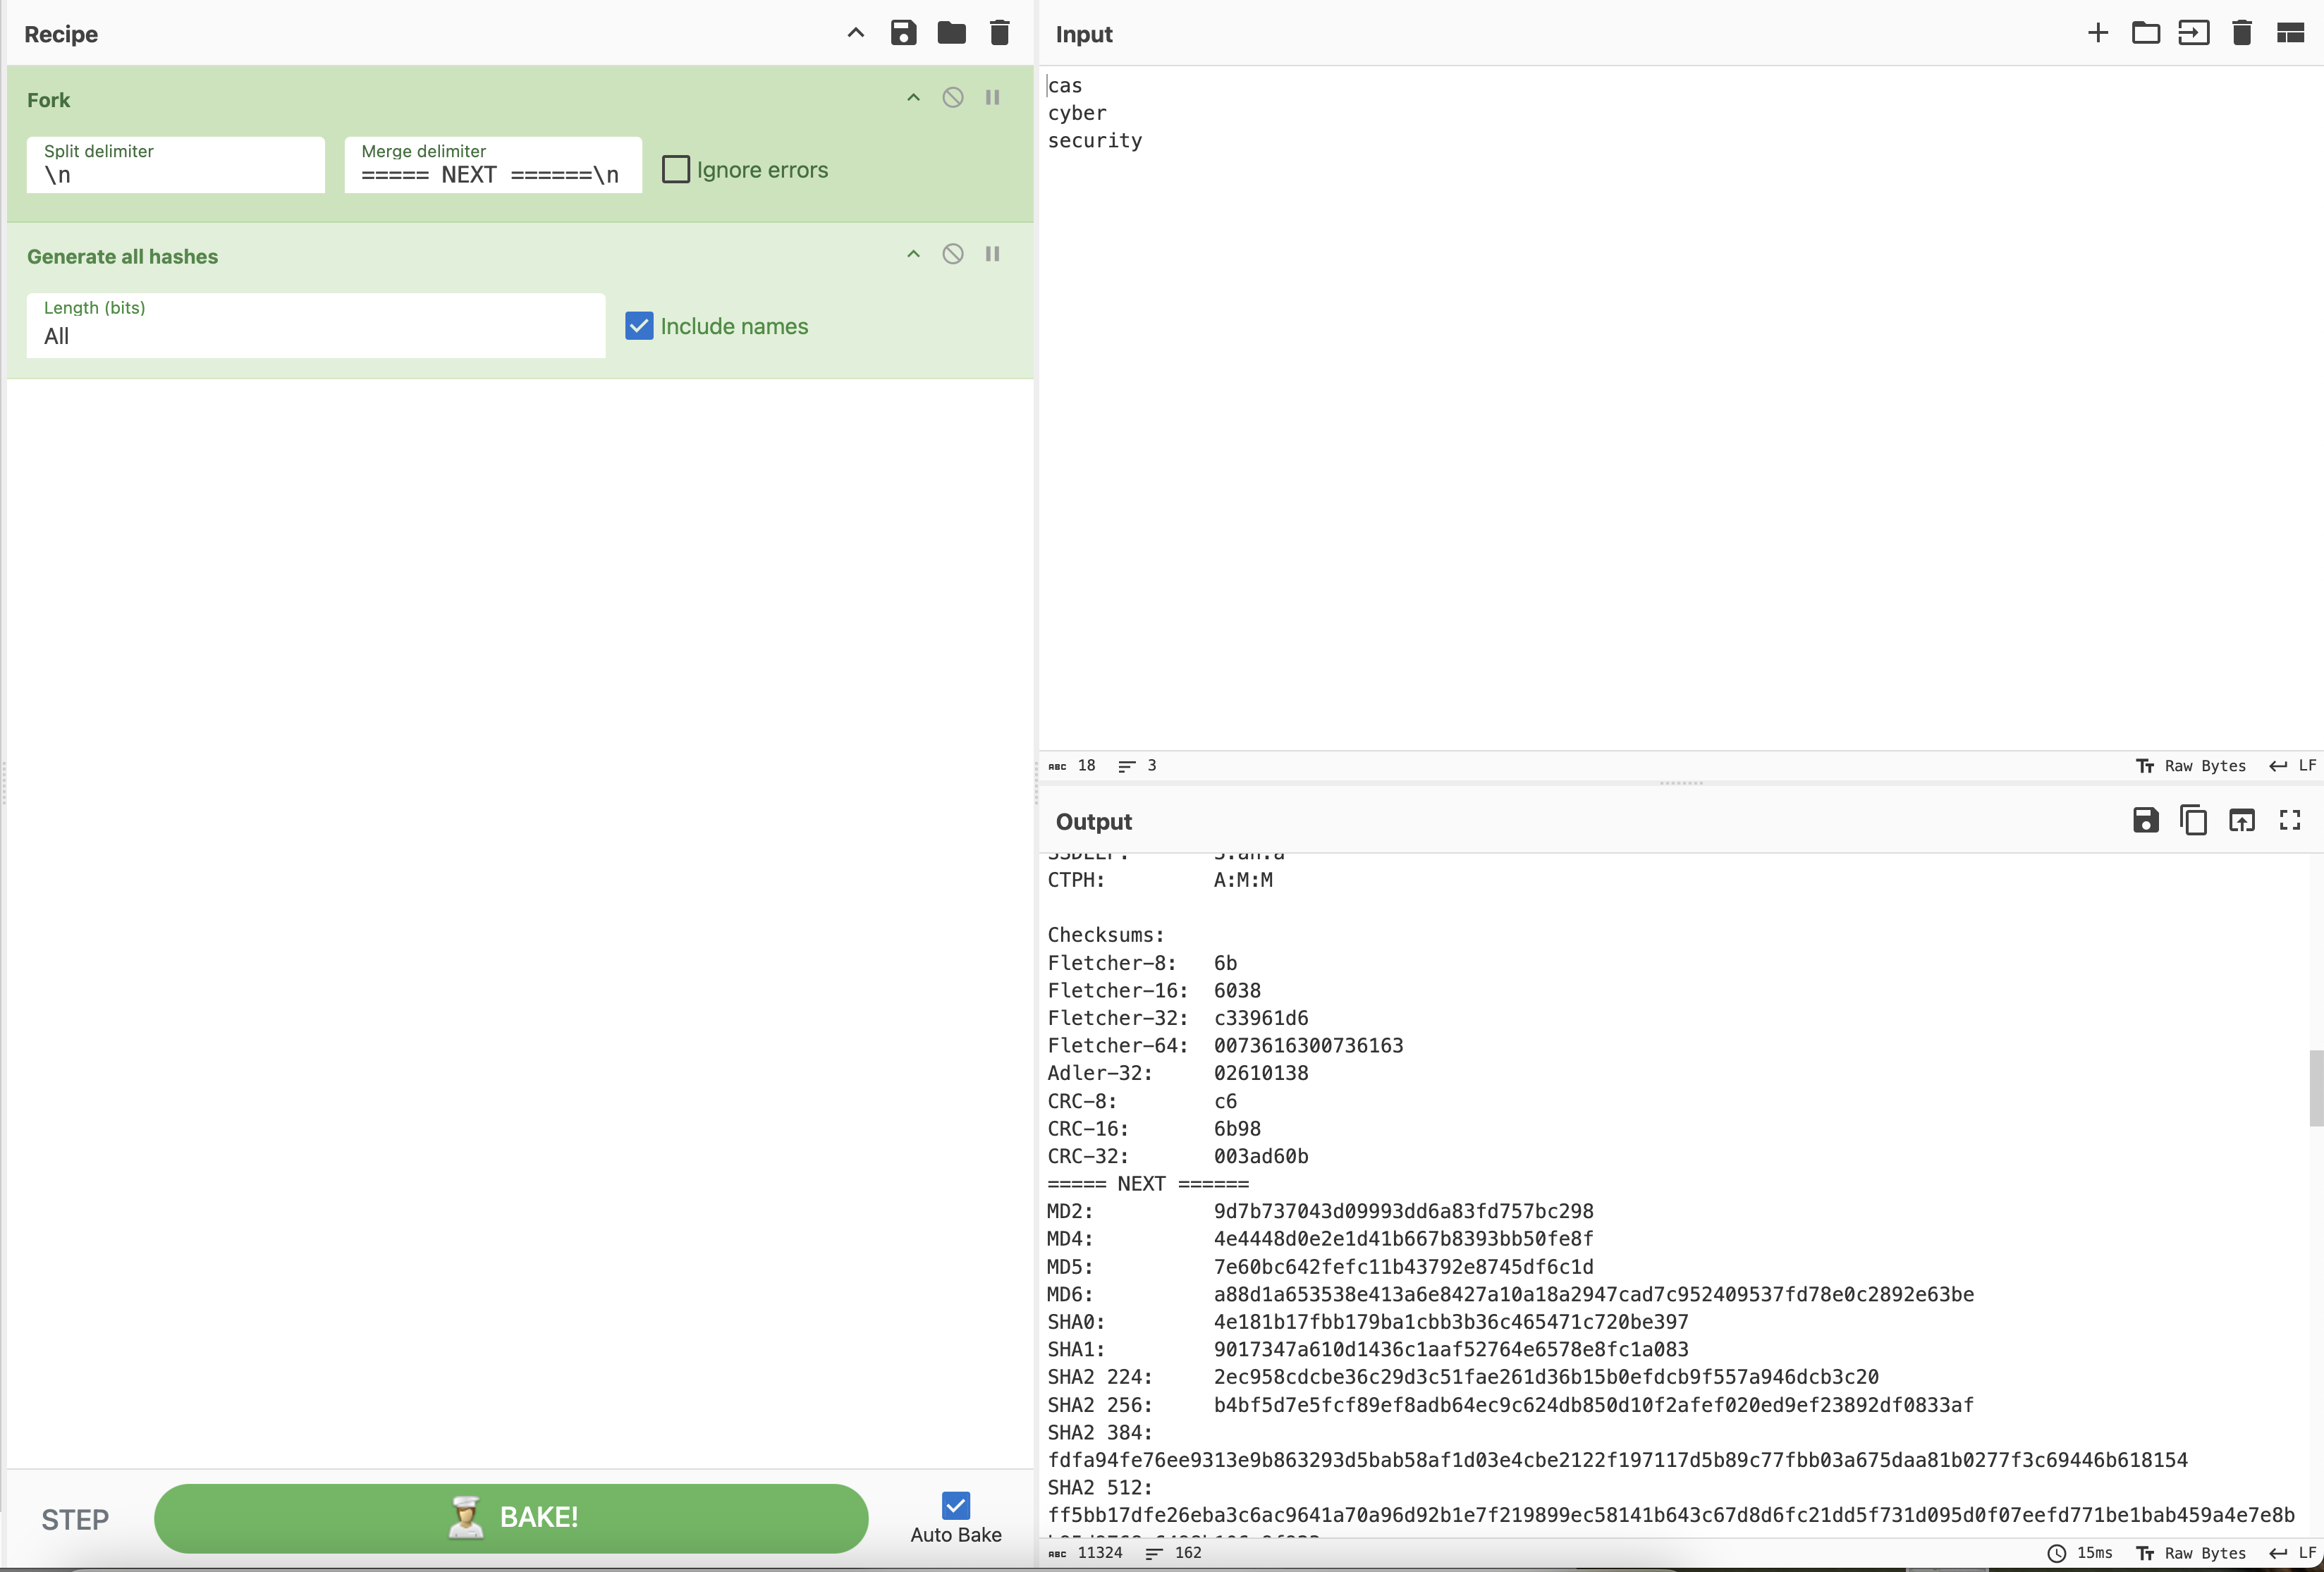
\includegraphics[width=0.8\textwidth]{resources/01_forking_CyberChef.png}
    \caption{Forking in CyberChef}
    \label{fig:forking}
\end{figure}

\textbf{JSON Recipe:}
\begin{lstlisting}[language=json,caption=Forking JSON Recipe]
[
  { "op": "Fork",
    "args": ["\\n", "===== NEXT ======\\n", false] },
  { "op": "Generate all hashes",
    "args": ["All", true] }
]
\end{lstlisting}

\subsubsection{HTTP Request and Email Extraction}
\textbf{Task:} Extract email addresses from multiple pages (pages 1-5).

\textbf{Methodology:}
\begin{enumerate}
    \item Used \emph{HTTP request} to fetch content from each page.
    \item Applied \emph{Extract email addresses} operation to identify unique emails.
\end{enumerate}

\textbf{Results:} A total of 27 email addresses were extracted: 8 from pages 1-4 and 3 from page 5.

\textbf{JSON Recipe:}
\begin{lstlisting}[language=json,caption=HTTP Request and Email Extraction Recipe]
[
  { "op": "Fork",
    "args": ["\\n", "\\n\\n", false] },
  { "op": "Register",
    "args": ["(.*)", true, false, false] },
  { "op": "HTTP request",
    "args": ["GET", "https://mcs.unibnf.ch/lecturers-list/page/$R0/", "", "Cross-Origin Resource Sharing", false] },
  { "op": "Extract email addresses",
    "args": [false, false, true] }
]
\end{lstlisting}

\subsubsection{Base64 Conversion and Malware Analysis}
\textbf{Steps:}
\begin{enumerate}
    \item Decoded Base64 content to readable text.
    \item Removed null values and dots to clean up the output.
\end{enumerate}

\textbf{Malware Behavior:}
\begin{enumerate}
    \item Created a WebClient object to download data.
    \item Set a fake user-agent string mimicking Internet Explorer.
    \item Configured proxy settings and system credentials.
    \item Downloaded and decrypted malicious data using XOR and a predefined key.
    \item Executed the decrypted data using \texttt{Invoke-Expression} (\texttt{IEX}).
\end{enumerate}

\textbf{Expected Output:} Figure~\ref{fig:malware} shows the expected result after decoding.

\begin{figure}[h!]
    \centering
    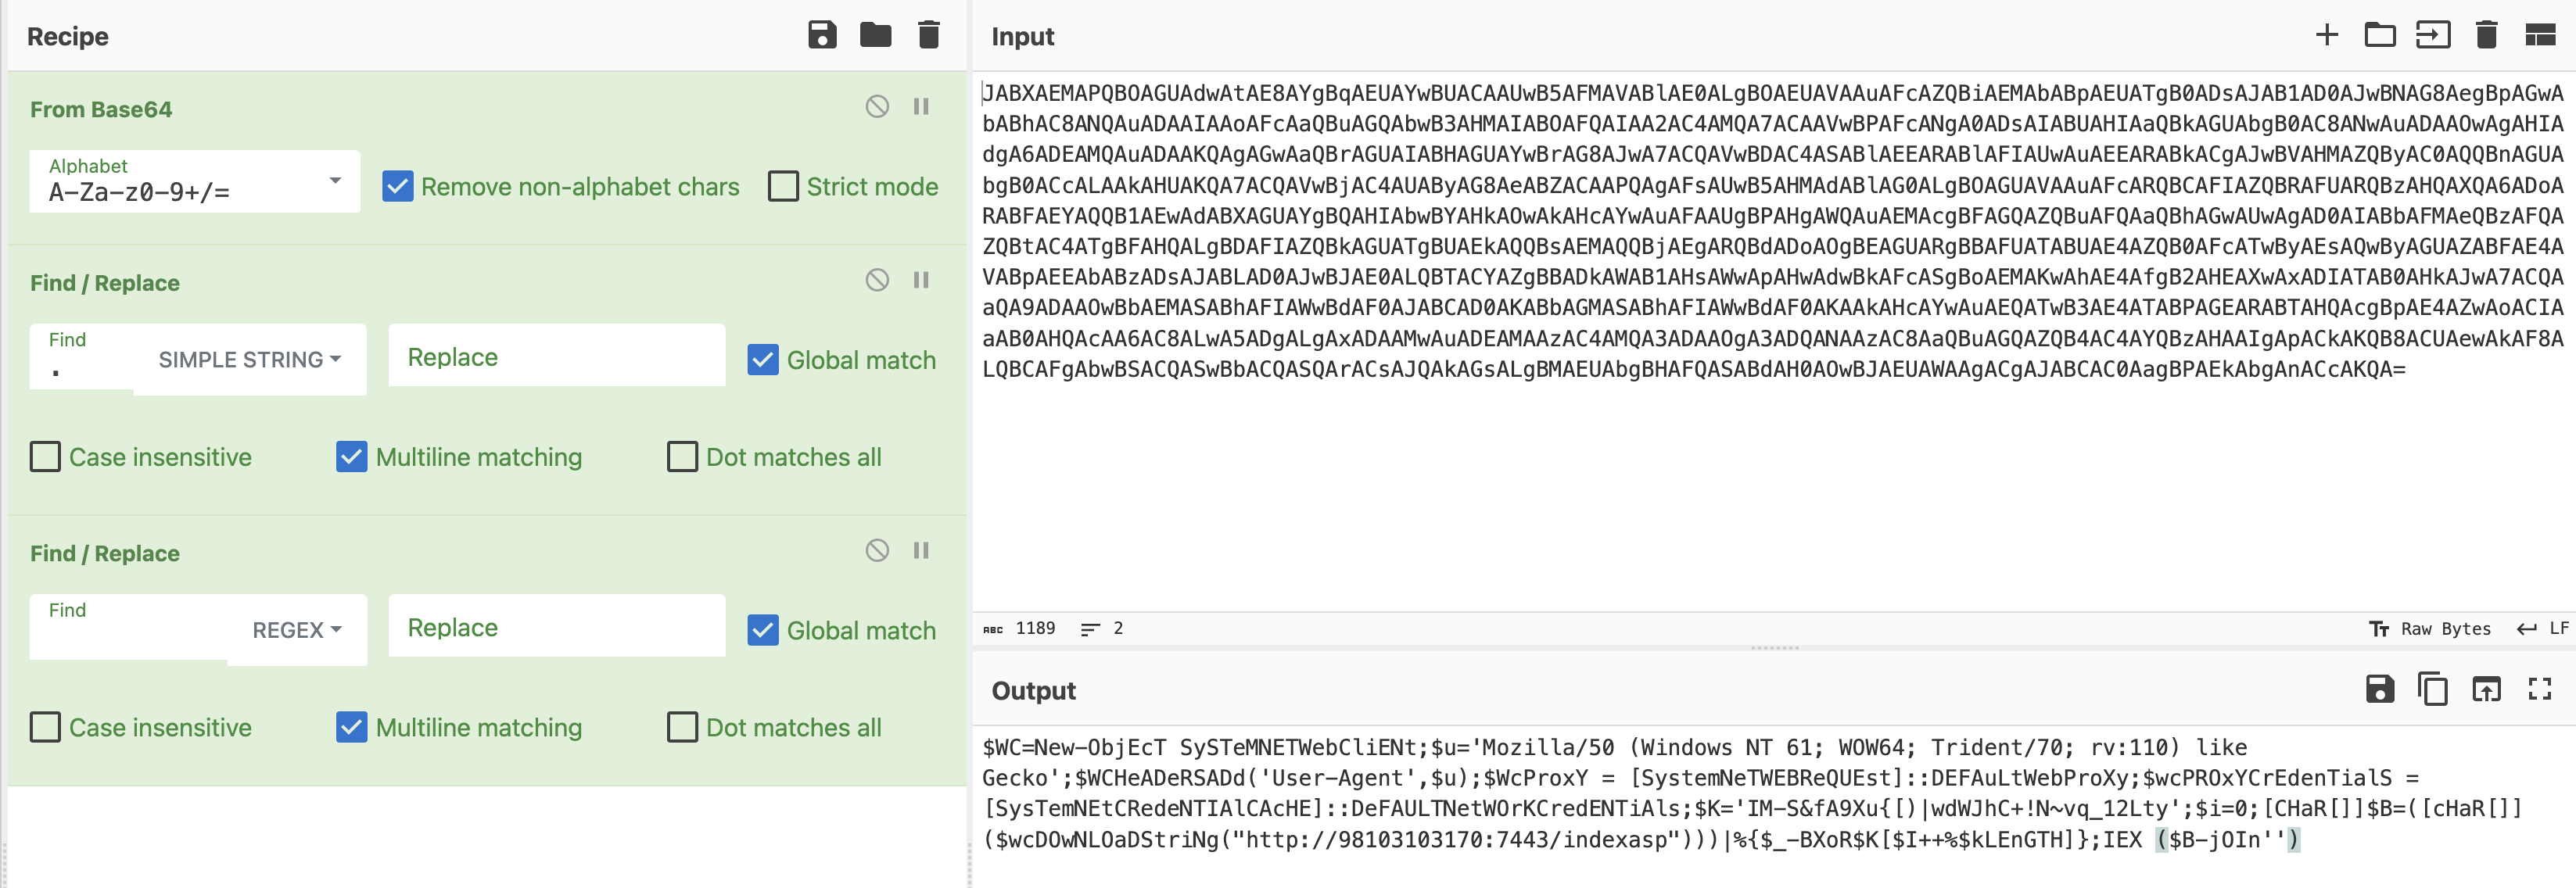
\includegraphics[width=0.8\textwidth]{resources/01_cyberchef.png}
    \caption{Base64 Decoding and Malware Analysis}
    \label{fig:malware}
\end{figure}

\subsection{Conclusion}
CyberChef is a versatile tool that can be effectively used for a variety of tasks, including data manipulation, decoding, and security analysis. Through its intuitive interface and flexibility, it simplifies otherwise complex operations.


\subsection{Regex}

\begin{center}
    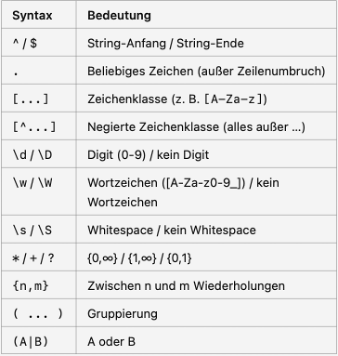
\includegraphics[scale=1]{resources/01_regex.png}
\end{center}

\begin{enumerate}
    \item \textbf{Allow only numbers} \\
    Solution: \verb|^[0-9]+$|
    
    \item \textbf{Allow only letters (A-Z, a-z) and a minimum length of 3 characters} \\
    Solution: \verb|^[A-Za-z]{3,}$|
    
    \item \textbf{Allow only alphanumeric characters and underscores} \\
    Solution: \verb|^[A-Za-z0-9_]+$| or \verb|^\w+$|
    
    \item \textbf{Allow an email address, but specify a regex that is as specific as possible} \\
    Solution: \verb|^[A-Za-z0-9._\%+-]+@[A-Za-z0-9.-]+\.[A-Za-z]{2,}$|
\end{enumerate}


\subsection{Lecture}
barfoo
